\documentclass[conference]{IEEEtran}
\IEEEoverridecommandlockouts
% The preceding line is only needed to identify funding in the first footnote. If that is unneeded, please comment it out.
\usepackage{cite}
\usepackage{amsmath,amssymb,amsfonts}
\usepackage{algorithmic}
\usepackage{graphicx}
\usepackage{textcomp}
\usepackage{xcolor}

% Tikz package for flowchart
\usepackage{tikz}
\usetikzlibrary{shapes.geometric, arrows}

\tikzstyle{startstop} = [rectangle, rounded corners, minimum width=3cm, minimum height=1cm,text centered, draw=black, fill=red!30]
\tikzstyle{process} = [rectangle, minimum width=3cm, minimum height=1cm, text centered, draw=black, fill=blue!20]
\tikzstyle{decision} = [diamond, minimum width=3cm, minimum height=1cm, text centered, draw=black, fill=yellow!30]
\tikzstyle{arrow} = [thick,->,>=stealth]

\def\BibTeX{{\rm B\kern-.05em{\sc i\kern-.025em b}\kern-.08em
    T\kern-.1667em\lower.7ex\hbox{E}\kern-.125emX}}
\begin{document}

\title{ECG Classification}
\author{\IEEEauthorblockN{
    %\IEEEauthorblockN{1\textsuperscript{st} Lewis G. Richter}
    \IEEEauthorblockN{Lewis G. Richter}
    \IEEEauthorblockA{\textit{AI \& Automation} \\
    \textit{University West}\\
    Trollhättan, Sweden \\
    lewis.richter@student.hv.se}
}}

\maketitle

\begin{abstract}
Insert abstract here.
\end{abstract}

\begin{IEEEkeywords}
Insert keywords here.
\end{IEEEkeywords}

\section{Administrative Details}
The project is a part of the course ``Deep Learning'' in the masters degree of ``Artificial Intelligence and Automation'' at University West, Trollhättan, Sweden. The project is supervised by Dr. Amit Kumar. The project is carried out by Lewis G. Richter.

The project files are available on \textit{GitHub} at \textit{https://github.com/RichLewi/ECGClassification.git}.

The project is effected by the EU Artificial Intelligence Regulations (EU) as it regulates AI applications based on a risk-based approach. Since ECG classification involves medical data and health diagnosis, it may fall under the category of high-risk AI systems due to its potential impact on people's health and safety. Compliance with the regulations requires ensuring data privacy and compliance with the General Data Protection Regulation (GDPR), ensuring transparency and traceability, and ensuring human oversight and accountability to avoid bias and discrimination. Before deploying the AI system, it is necessary to conduct a risk assessment and ensure that the system follows medical certification standards. 

\section{Requirement and Data Analysis}
In this project, a deep learning model for ECG heartbeat classification is developed, different AI models are compared and evaluated based on their accuracy and loss. The model should be able to classify ECG heartbeats into five classes. The model should achieve an accuracy of at least 95\% on the testing set. Performance metrics such as accuracy, precision, recall, and F1-score are used to evaluate the model and should perform robust across different patients and avoid overfitting.
The EU regulations regarding medical AI need to be considered, therefor GDPR compliance should be met when handling patient data. 

The dataset used in this project originates from Kaggle's ECG Heartbeat Categorization Dataset. The dataset contains 109446 ECG heartbeats, each labeled as one of the five classes: Normal, Supraventricular, Ventricular, Fusion, and Unknown. The dataset is divided into training and testing sets. The training set contains 87554 samples, and the testing set contains 21890 samples. The dataset is imbalanced, with the Normal class having the most samples and the Fusion class having the least samples. 

Next we visualize the dataset distribution and some samples of the ECG heartbeats of each class. In figure \ref{fig:dataset_distribution}, the dataset distribution is shown. In figure \ref{fig:ecg_samples}, some samples of the ECG heartbeats of each class are shown.

\begin{figure}[htbp]
    \centering
    \includegraphics[width=0.5\textwidth]{images/distribution-classes-bar.png}
    \caption{Dataset Distribution}
    \label{fig:dataset_distribution}
\end{figure}

\begin{figure}[htbp]
    \centering
    \includegraphics[width=0.5\textwidth]{images/one-ecg-per-class.png}
    \caption{ECG Heartbeat Samples}
    \label{fig:ecg_samples}
\end{figure}


\section{System Engineering}
In this chapter, the system implementation is described using the flow chart from figure \ref{fig:flowchart}. The system consists of the following steps: data preprocessing, model training, model evaluation. The data preprocessing step involves loading the dataset, splitting the dataset into training, validation and testing sets. The data of training and validation set are normalized and balanced. The model training step involves building the deep learning models, training the models on the training set, and saving the model. The model evaluation step involves evaluating the model on the testing set and calculating the accuracy and loss. 

\begin{figure}
    \begin{center}
        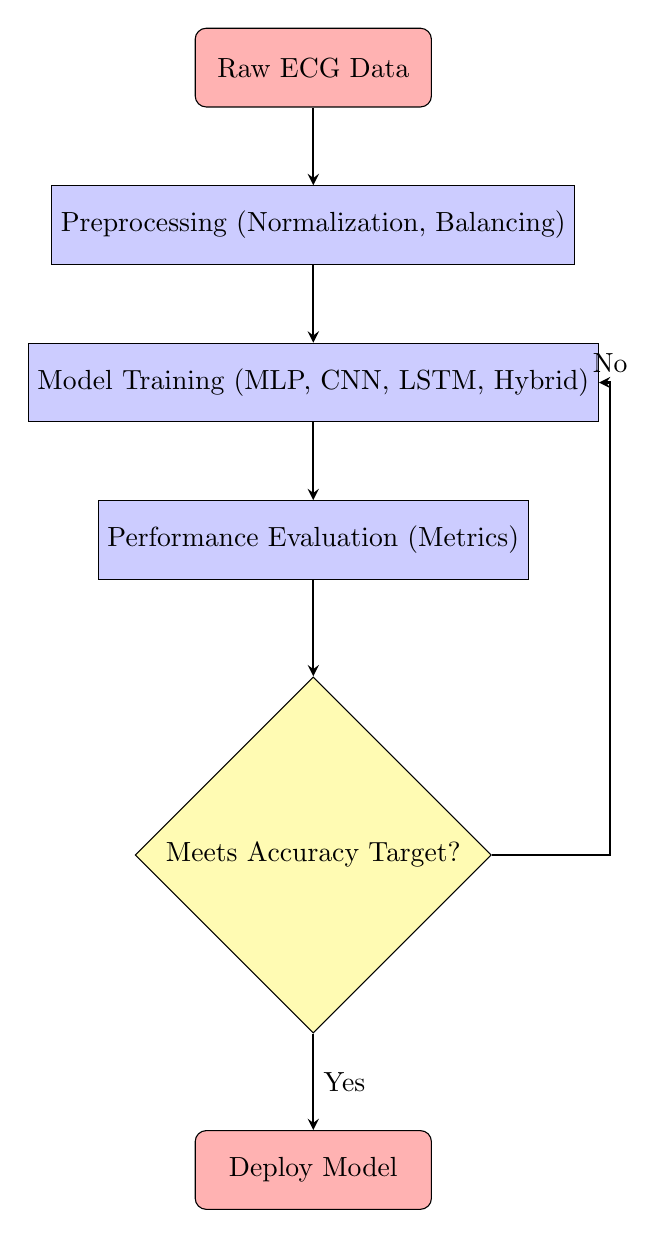
\begin{tikzpicture}[node distance=2cm]
            \node (start) [startstop] {Raw ECG Data};
            \node (preprocess) [process, below of=start] {Preprocessing (Normalization, Balancing)};
            \node (model) [process, below of=preprocess] {Model Training (MLP, CNN, LSTM, Hybrid)};
            \node (evaluate) [process, below of=model] {Performance Evaluation (Metrics)};
            \node (decision) [decision, below of=evaluate, yshift=-2cm] {Meets Accuracy Target?};
            \node (end) [startstop, below of=decision, yshift=-2cm] {Deploy Model};
            
            \draw [arrow] (start) -- (preprocess);
            \draw [arrow] (preprocess) -- (model);
            \draw [arrow] (model) -- (evaluate);
            \draw [arrow] (evaluate) -- (decision);
            \draw [arrow] (decision.east) -- ++(1.5,0) |- (model.east) node[midway,above] {No};
            %\draw [arrow] (evaluate.north) |- (model.east);
            \draw [arrow] (decision.south) -- (end) node[midway, right] {Yes};
        \end{tikzpicture}
    \end{center}
    \caption{Flowchart of the System}
    \label{fig:flowchart}
\end{figure}



\section{Algorithm Design Using Spiral Approach}

\section{Performance Evaluation}

\section{Conclusion}

\section*{Acknowledgment}

\bibliographystyle{IEEEtran}
\bibliography{Insert your bibliography file here}

\begin{thebibliography}{00}
    \bibitem{b1} G. Eason, B. Noble, and I. N. Sneddon, ``On certain integrals of Lipschitz-Hankel type involving products of Bessel functions,'' Phil. Trans. Roy. Soc. London, vol. A247, pp. 529--551, April 1955.
    \bibitem{b2} “Regulation - EU - 2024/1689 - EN - EUR-LEX.” https://eur-lex.europa.eu/legal-content/EN/TXT/?uri=CELEX\%3A32024R1689 (accessed Dec. 02, 2021).
\end{thebibliography}

\end{document}